\section{Fuselage}

\begin{tabularx}{\textwidth}{ | L | c | c | }
  \hline
  \textbf{Parameter}                    & \textbf{Value}   & \textbf{Reference} \\ \hline
  \endfirsthead
  \hline
  \textbf{Parameter}                    & \textbf{Value}   & \textbf{Reference} \\ \hline
  \endhead
  Fuselage length                       & 15.26 m          & \cite{Janes20042005,NASA-CR-166309} \\ \hline
  Fuselage width                        & 2.36 m           & \cite{UH60_OperatorsManual,Janes20042005} \\ \hline
  Fuselage aerodynamic reference point stationline & 8.78 m & \cite{NASA-CR-166309,NASA-TM-85890} \\ \hline
  Fuselage aerodynamic reference point waterline   & 5.94 m & \cite{NASA-CR-166309,NASA-TM-85890} \\ \hline
  \caption{Fuselage data}
\end{tabularx}

%%%%%%%%%%%%%%%%%%%%%%%%%%%%%%%%%%%%%%%%%%%%%%%%%%%%%%%%%%%%%%%%%%%%%%%%%%%%%%%%

\clearpage
\subsection{Symbols}

\begin{tabularx}{\textwidth}{ L l l l }
  \hline
  \textbf{Symbol} & \textbf{Mnemonic} & \textbf{Unit} & \textbf{Description} \\ \hline
  \endfirsthead
  \hline
  \textbf{Symbol} & \textbf{Mnemonic} & \textbf{Unit} & \textbf{Description} \\ \hline
  \endhead
  $EK_{XWF}$     & EKXWF  & -     & Rotor wash interference factor (inplane) \\
  $EK_{YWF}$     & EKYWF  & -     & Rotor wash interference factor (sidewash) \\
  $EK_{ZWF}$     & EKZWF  & -     & Rotor wash interference factor (downwash) \\
  & & & \\
  $\chi_{PMR}$   & CHIPMR & deg   & Rotor wake skew angle \\
  $D_{WO}$       & DWSHMR & -     & Main rotor uniform downwash \\
  $\Omega_T$     & OMGTMR & rad/s & Rotor speed \\
  $R_T$          & RMR    & m     & Rotor radius \\
  & & & \\
  $q_{WF}$       & QWF    & Pa    & dynamic pressure at the body \\
  & & & \\
  $\alpha_{WF}$  & ALFWF  & deg   & angle of attack \\
  $\beta_{WF}$   & BETAWF & deg   & sideslip angle \\
  $\psi_{WF}$    & PSIWF  & deg   & W/T model yaw angle ($\psi_{WF} = -\beta_{WF}$) \\ \hline
  \caption{Fuselage symbols}
\end{tabularx}

%%%%%%%%%%%%%%%%%%%%%%%%%%%%%%%%%%%%%%%%%%%%%%%%%%%%%%%%%%%%%%%%%%%%%%%%%%%%%%%%

\clearpage
\subsection{Inplane Component of Rotor Wash on the Fuselage}

\csvreader[
  no head,
  longtable=cccc,
  table head=
    \toprule
    $\chi_{PMR}$ & \multicolumn{3}{c}{$EK_{XWF}$} \\
    {[deg]} & {AA1FMR=-6.0} & {AA1FMR=0.0} & {AA1FMR=6.0} \\ \midrule
    \endfirsthead
    $\chi_{PMR}$ & \multicolumn{3}{c}{$EK_{XWF}$} \\
    {[deg]} & {AA1FMR=-6.0} & {AA1FMR=0.0} & {AA1FMR=6.0} \\ \midrule
    \endhead,
  before first line={},
  late after line=\\,
  late after last line=\\ \bottomrule \caption{Inplane component of rotor wash on the fuselage \cite{NASA-CR-166309}},
  before reading={},
  after reading={}
]
{csv/uh60_fuselage_chipmr_ekxwf.csv}
{1=\colchi,2=\colii,3=\coliii,4=\coliv}
{\colchi & \colii & \coliii & \coliv}

\begin{figure}[h!]
  \centering
  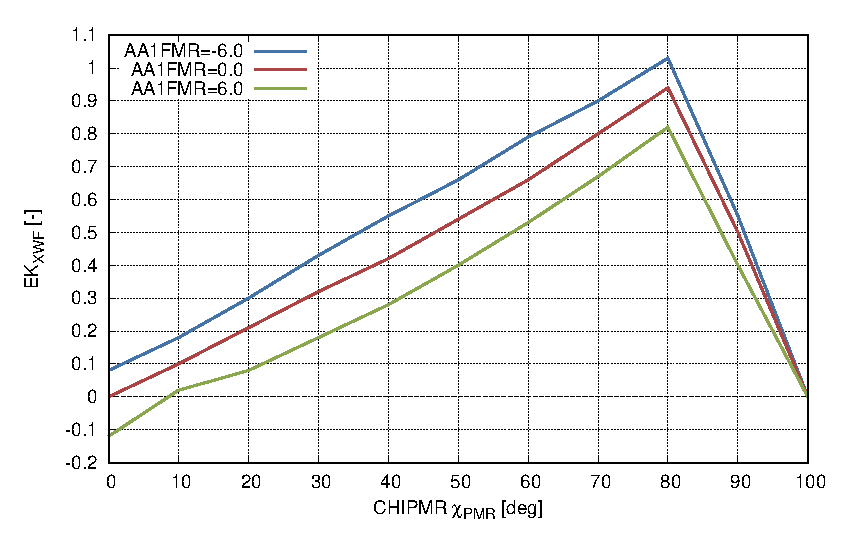
\includegraphics[width=140mm]{eps/uh60_fuselage_chipmr_ekxwf.eps}
  \caption{Inplane component of rotor wash on the fuselage \cite{NASA-CR-166309}}
\end{figure}

%%%%%%%%%%%%%%%%%%%%%%%%%%%%%%%%%%%%%%%%%%%%%%%%%%%%%%%%%%%%%%%%%%%%%%%%%%%%%%%%

\clearpage
\subsection{Downwash Component of Rotor Wash on the Fuselage}

\csvreader[
  no head,
  longtable=cccc,
  table head=
    \toprule
    $\chi_{PMR}$ & \multicolumn{3}{c}{$EK_{ZWF}$} \\
    {[deg]} & {AA1FMR=-6.0} & {AA1FMR=0.0} & {AA1FMR=6.0} \\ \midrule
    \endfirsthead
    $\chi_{PMR}$ & \multicolumn{3}{c}{$EK_{ZWF}$} \\
    {[deg]} & {AA1FMR=-6.0} & {AA1FMR=0.0} & {AA1FMR=6.0} \\ \midrule
    \endhead,
  before first line={},
  late after line=\\,
  late after last line=\\ \bottomrule \caption{Downwash component of rotor wash on the fuselage \cite{NASA-CR-166309}},
  before reading={},
  after reading={}
]
{csv/uh60_fuselage_chipmr_ekzwf.csv}
{1=\colchi,2=\colii,3=\coliii,4=\coliv}
{\colchi & \colii & \coliii & \coliv}

\begin{figure}[h!]
  \centering
  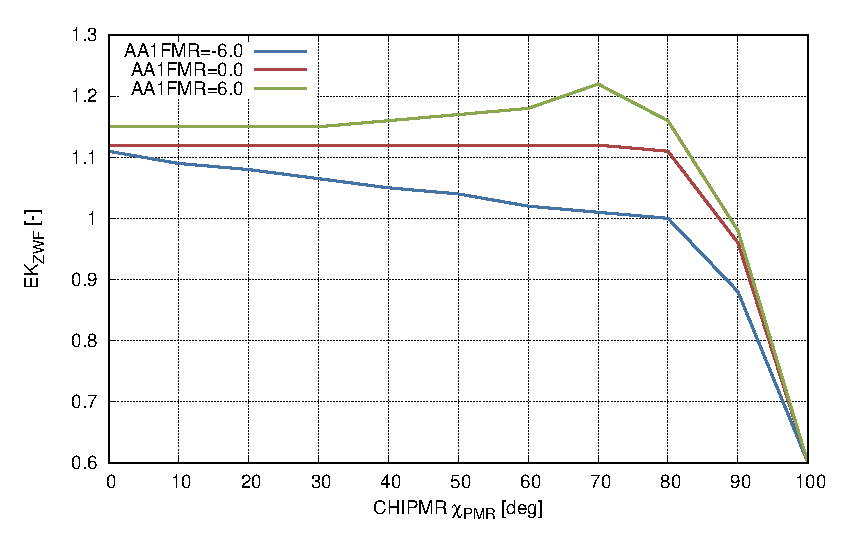
\includegraphics[width=140mm]{eps/uh60_fuselage_chipmr_ekzwf.eps}
  \caption{Downwash component of rotor wash on the fuselage \cite{NASA-CR-166309}}
\end{figure}

%%%%%%%%%%%%%%%%%%%%%%%%%%%%%%%%%%%%%%%%%%%%%%%%%%%%%%%%%%%%%%%%%%%%%%%%%%%%%%%%

\clearpage
\subsection{Basic Fuselage Aerodynamic Characteristics}

\csvreader[
  no head,
  longtable=cccc,
  table head=
    \toprule
    $\alpha_{WF}$ & $D/q$ & $L/q$ & $M/q$ \\
    {[deg]} & {[m\textsuperscript{2}]} & {[m\textsuperscript{2}]} & {[m\textsuperscript{3}]} \\ \midrule
    \endfirsthead
    $\alpha_{WF}$ & $D/q$ & $L/q$ & $M/q$ \\
    {[deg]} & {[m\textsuperscript{2}]} & {[m\textsuperscript{2}]} & {[m\textsuperscript{3}]} \\ \midrule
    \endhead,
  before first line={},
  late after line=\\,
  late after last line=\\ \bottomrule \caption{Fuselage aerodynamic characteristics due to angle of attack \cite{NASA-CR-166309}},
  before reading={},
  after reading={}
]
{csv/uh60_aero_fuselage_alfwf.csv}
{1=\colaoa,2=\colcx,3=\colcz,4=\colcm}
{\colaoa & \colcx & \colcz & \colcm}

\begin{figure}
  \centering
  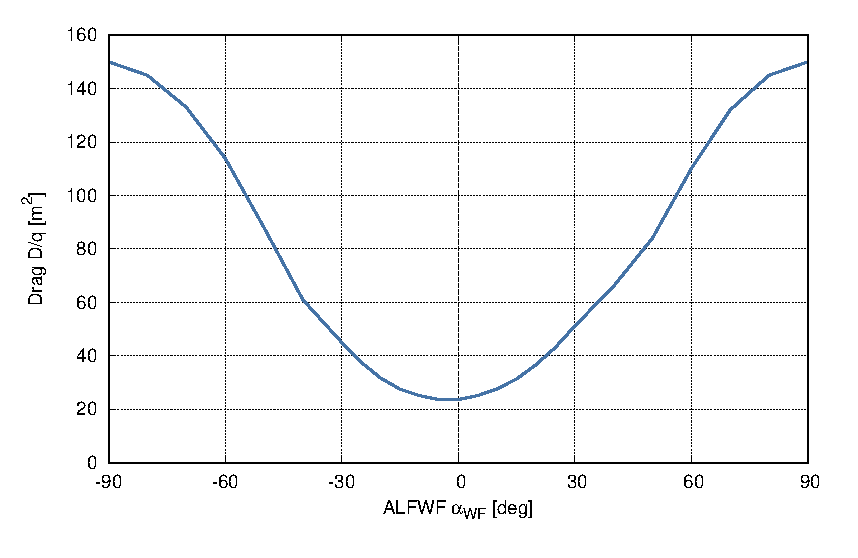
\includegraphics[width=140mm]{eps/uh60_fuselage_alfwf_dqfmp.eps}
  \caption{Fuselage drag due to angle of attack \cite{NASA-CR-166309}}
\end{figure}

\begin{figure}
  \centering
  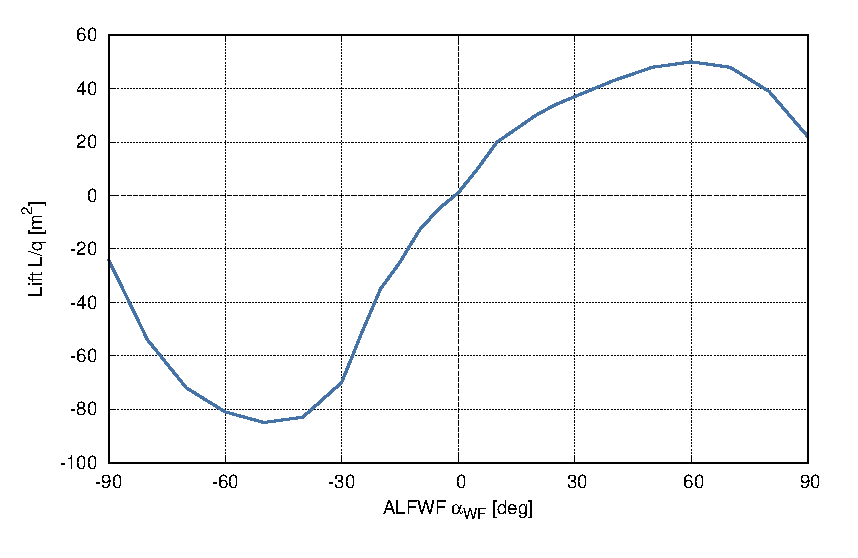
\includegraphics[width=140mm]{eps/uh60_fuselage_alfwf_lqfmp.eps}
  \caption{Fuselage lift due to angle of attack \cite{NASA-CR-166309}}
\end{figure}

\begin{figure}
  \centering
  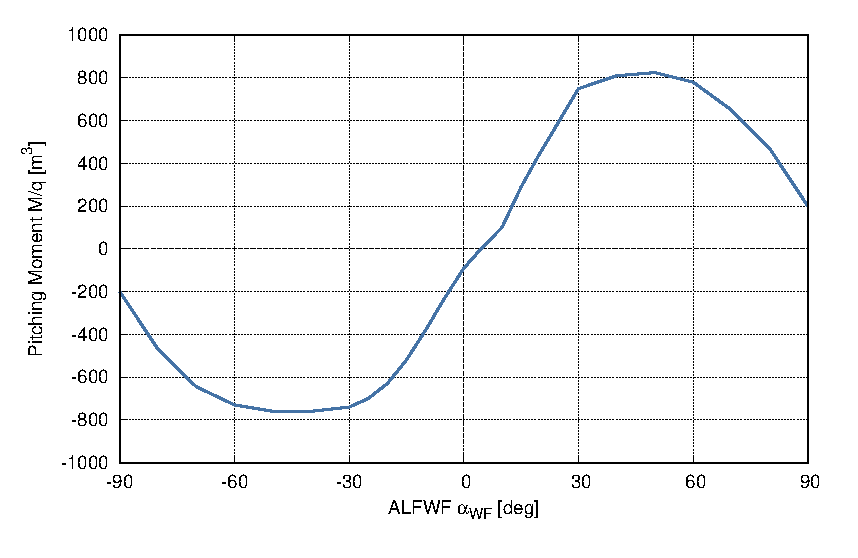
\includegraphics[width=140mm]{eps/uh60_fuselage_alfwf_mqfmp.eps}
  \caption{Fuselage pitching moment due to angle of attack \cite{NASA-CR-166309}}
\end{figure}

\clearpage

\csvreader[
  no head,
  longtable=cccc,
  table head=
    \toprule
    $\psi_{WF}$ & $Y/q$ & $R/q$ & $N/q$ \\
    {[deg]} & {[m\textsuperscript{2}]} & {[m\textsuperscript{3}]} & {[m\textsuperscript{3}]} \\ \midrule
    \endfirsthead
    $\psi_{WF}$ & $Y/q$ & $R/q$ & $N/q$ \\
    {[deg]} & {[m\textsuperscript{2}]} & {[m\textsuperscript{3}]} & {[m\textsuperscript{3}]} \\ \midrule
    \endhead,
  before first line={},
  late after line=\\,
  late after last line=\\ \bottomrule \caption{Fuselage aerodynamic characteristics due to sideslip \cite{NASA-CR-166309}},
  before reading={},
  after reading={}
]
{csv/uh60_aero_fuselage_psiwf.csv}
{1=\colbeta,2=\colcy,3=\colcl,4=\colcn,5=\coldcx}
{\colbeta & \colcy & \colcl & \colcn}

\begin{figure}
  \centering
  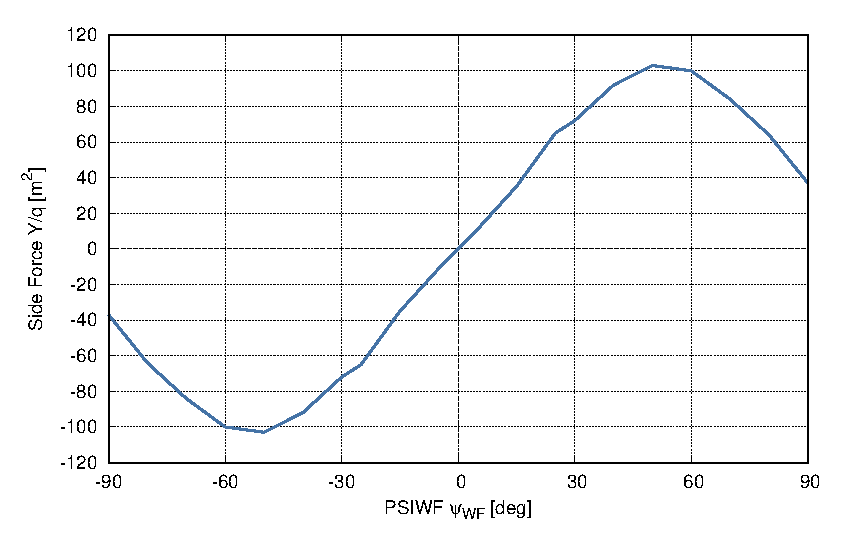
\includegraphics[width=140mm]{eps/uh60_fuselage_psiwf_yqfmp.eps}
  \caption{Fuselage side force due to sideslip \cite{NASA-CR-166309}}
\end{figure}

\begin{figure}
  \centering
  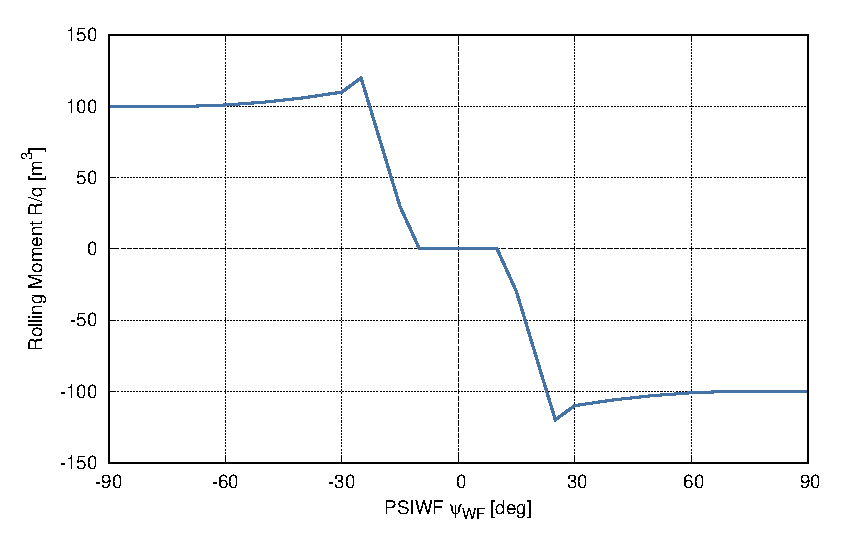
\includegraphics[width=140mm]{eps/uh60_fuselage_psiwf_rqfmp.eps}
  \caption{Fuselage rolling moment due to sideslip \cite{NASA-CR-166309}}
\end{figure}

\begin{figure}
  \centering
  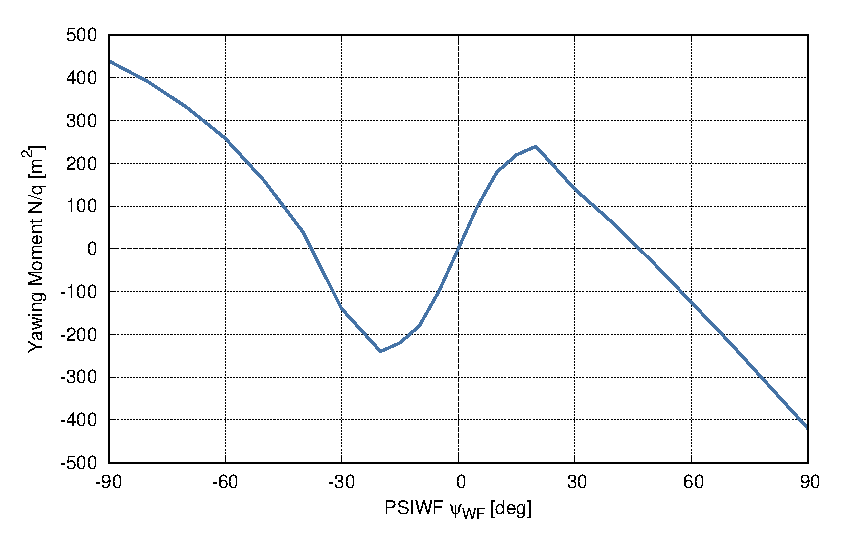
\includegraphics[width=140mm]{eps/uh60_fuselage_psiwf_nqfmp.eps}
  \caption{Fuselage yawing moment due to sideslip \cite{NASA-CR-166309}}
\end{figure}

%%%%%%%%%%%%%%%%%%%%%%%%%%%%%%%%%%%%%%%%%%%%%%%%%%%%%%%%%%%%%%%%%%%%%%%%%%%%%%%%

\clearpage
\subsection{Fuselage Incremental Aerodynamic Characteristics}

\csvreader[
  no head,
  longtable=cccc,
  table head=
    \toprule
    $\psi_{WF}$ & $\Delta D/q$ & $\Delta L/q$ & $\Delta M/q$ \\
    {[deg]} & {[m\textsuperscript{2}]} & {[m\textsuperscript{2}]} & {[m\textsuperscript{3}]} \\ \midrule
    \endfirsthead
    $\psi_{WF}$ & $\Delta D/q$ & $\Delta L/q$ & $\Delta M/q$ \\
    {[deg]} & {[m\textsuperscript{2}]} & {[m\textsuperscript{2}]} & {[m\textsuperscript{3}]} \\ \midrule
    \endhead,
  before first line={},
  late after line=\\,
  late after last line=\\ \bottomrule \caption{Fuselage incremental aerodynamic characteristics \cite{NASA-CR-166309}},
  before reading={},
  after reading={}
]
{csv/uh60_aero_fuselage_psiwf3.csv}
{1=\colbeta,2=\coldcx,3=\coldcz,4=\coldcm}
{\colbeta & \coldcx & \coldcz & \coldcm}

\begin{figure}
  \centering
  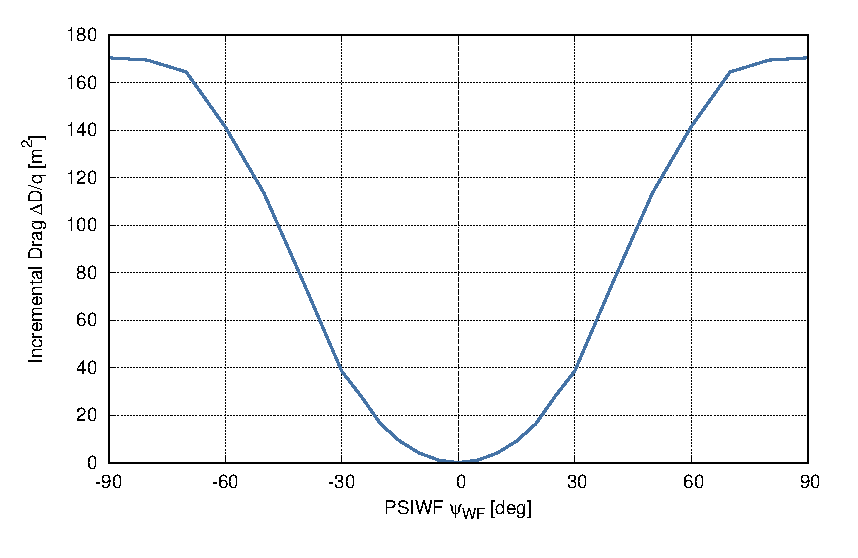
\includegraphics[width=140mm]{eps/uh60_fuselage_psiwf_ddqfmp.eps}
  \caption{Fuselage incremental drag due to sideslip \cite{NASA-CR-166309}}
\end{figure}

\begin{figure}
  \centering
  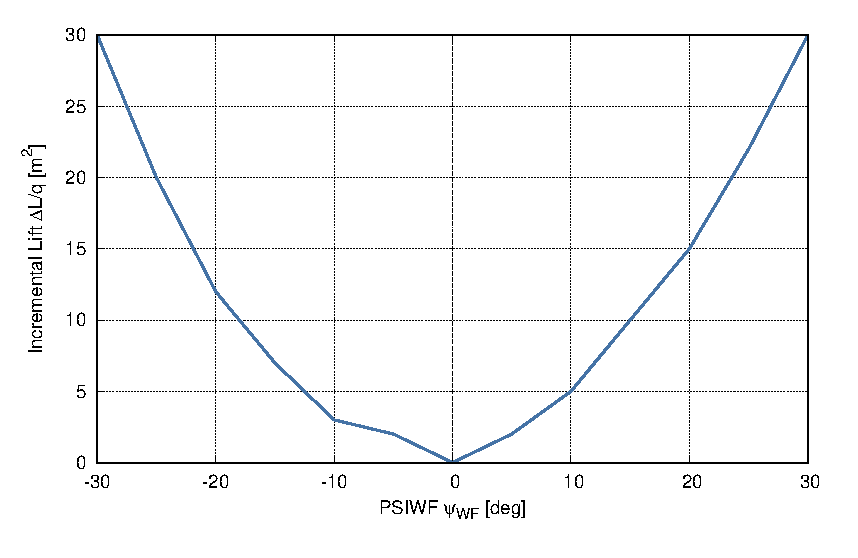
\includegraphics[width=140mm]{eps/uh60_fuselage_psiwf_dlqfmp.eps}
  \caption{Fuselage incremental lift due to sideslip \cite{NASA-CR-166309}}
\end{figure}

\begin{figure}
  \centering
  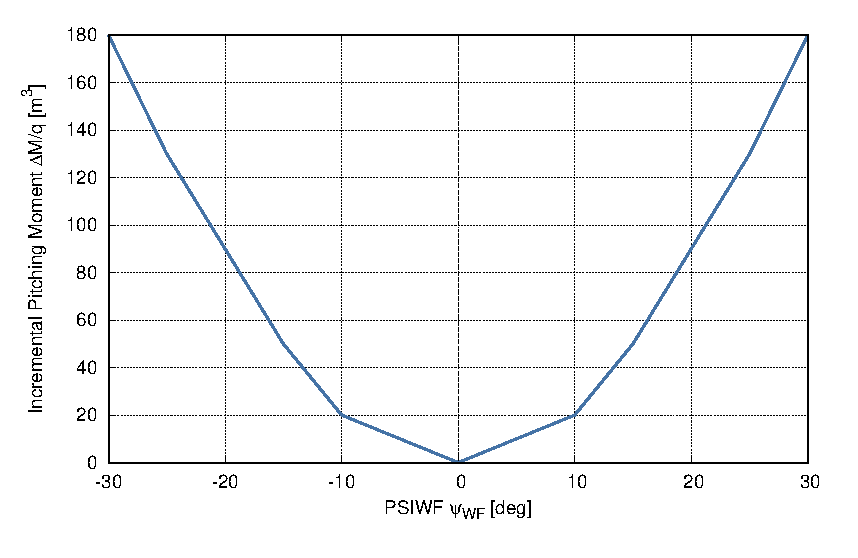
\includegraphics[width=140mm]{eps/uh60_fuselage_psiwf_dmqfmp.eps}
  \caption{Fuselage incremental pitching moment due to sideslip \cite{NASA-CR-166309}}
\end{figure}
